\section{Data}\label{sec:data} 

Both Mannequin Challenge~\cite{li2019learning} and RealEstate10K~\cite{zhou2018stereo} datasets were created by roughly the same group of researchers hailing from Google. They involved the same ORB-SLAM2, COLMAP, and scale-normalization procedures as Zhou et al.~\cite{zhou2018stereo} (Subsection~\ref{subsec:base-papers}). Hence, both datasets consist of the same kind of metadata in text files pertaining to the downloadable videos. Each text file begins with the video’s YouTube link on the first line and continues with the details of each COLMAP-processed video frame from the second line onward. Frame details include the timestamp (in microseconds), camera intrinsics, and camera extrinsics. As mentioned in subsection~\ref{subsec:base-papers}, COLMAP consists of a 3D scene reconstruction pipeline. It attempts to recover the 3D scene structure from even those unstructured 2D images of the scene that do not come tagged with any prior knowledge of camera intrinsics, extrinsics, and the nature of objects captured. The extracted scene structure is either in the form of sparse 3D points along with the camera parameters for each input 2D image or dense 3D points with associated color information. COLMAP's pipeline can be given by: feature detection $\rightarrow$ pairwise feature matching  $\rightarrow$ correspondence estimation $\rightarrow$ incremental structure from motion (Figure~\ref{fig:colmap-photogrammetry-pipeline}). Fortunately, the model does not require absolute camera poses; only the relative ones made available with the help of COLMAP in these text files are needed. Our scripts to download and curate all these videos were facilitated by our compilation of a comprehensive Docker container ensuring robustness in code reusability and transferability. Resolving version compatibility issues among our project dependencies, such as COLMAP and OpenFace 2.2, both in the Docker container and in Google Colaboratory, proved paramount to the successful running of our experiments. All our scripts, notebooks, sample renderings, demos, and most other aspects of our code for this project can be found in our GitHub repository (Section~\ref{sec:code-sources}).

\begin{figure}[!h]
    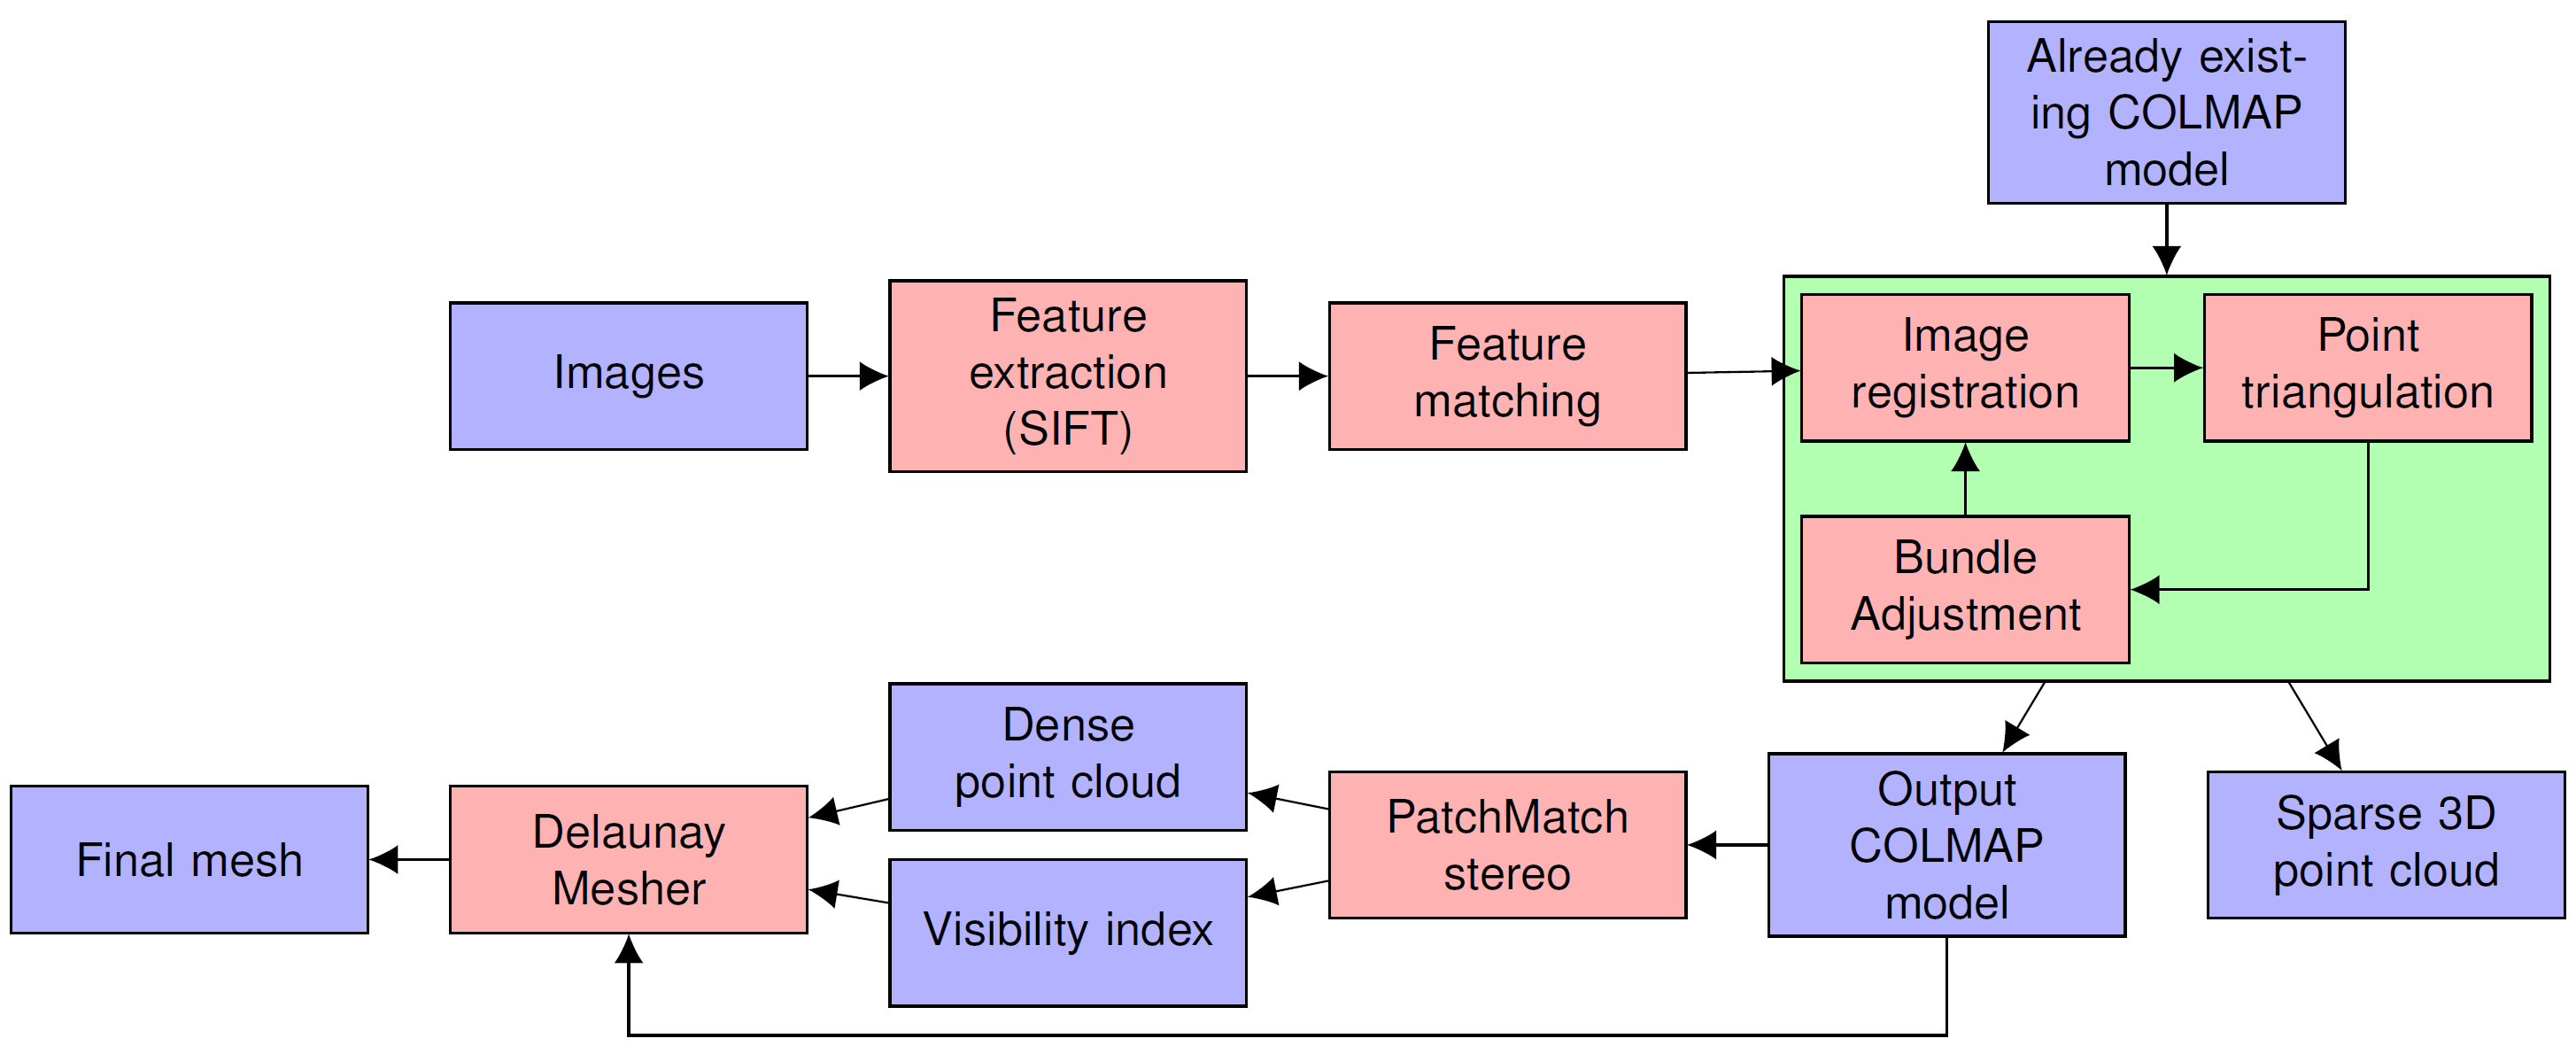
\includegraphics[width=1\columnwidth]{figures/colmap-photogrammetry-pipeline.png}
    \caption{Photogrammetry Workflow Used in COLMAP~\cite{pinard_does_2021}}
    \label{fig:colmap-photogrammetry-pipeline}
\end{figure}
    
Although our training and testing scripts are designed to crop all incoming video frames to 512$\times$512 pixels, we ensured that we downloaded all videos with youtube-dl at 720p resolution. This uniformity was so we could reduce the number of sources of arbitrariness in the initial process of replicating Tucker and Snavely's~\cite{single_view_mpi} work. Linking youtube-dl with the download management utility aria2~\cite{noauthor_aria2_2021} proved very useful in bolstering youtube-dl’s download speed by optimizing resource utilization. We then targeted addressing youtube-dl download errors. There would inevitably be several partial and/or skipped downloads for various reasons ranging from the videos being taken down from YouTube over time to fixable errors intrinsic to youtube-dl. Moreover, some videos were unavailable in their 720p versions and were discarded by us to maintain consistency. In favor of retaining the pristine versions, we chose not to manually convert the varying resolutions to 720p. Although differently scaled videos should theoretically not pose any problem to training or 3D point cloud generation with COLMAP, we opted again to go with uniformity and consequent ease of reproducibility for one and all.
    
We were finally able to procure 66861 RealEstate10K videos with 9095528 frames and 2364 MannequinChallenge videos with 117811 frames for processing. However, not all downloaded videos could be processed. For instance, only $\sim$60000 RealEstate10K videos were actually COLMAP-processed and used for training. The rest of the videos did not meet COLMAP processing requirements. Moreover, it would have taken 200 days to process all 66861 videos with COLMAP with CPUs alone. Fortunately, we could avail the benefits of NVIDIA Tesla V100 GPUs (rated the best server models in 2020) at Cal Poly and could bring down the processing time to 25 days. In these ways, we obtained the required point clouds and frames for training and testing.















